\documentclass[11pt,a4paper,openany]{book}

\usepackage[T1]{fontenc}
\usepackage[utf8]{inputenc}
\usepackage[english]{babel}
\usepackage{lmodern}
\usepackage{microtype}
\usepackage[a4paper,margin=2.35cm,headheight=15pt]{geometry}
\usepackage{graphicx}
\usepackage{booktabs}
\usepackage{tabularx}
\usepackage{longtable}
\usepackage{array}
\usepackage{enumitem}
\usepackage{xcolor}
\usepackage{amsmath,amssymb,mathtools}
\usepackage{tikz}
\usetikzlibrary{arrows.meta,positioning,fit,calc,shapes.geometric}
\usepackage[most]{tcolorbox}
\usepackage{listings}
\usepackage{caption}
\usepackage{subcaption}
\usepackage{float}
\usepackage[section]{placeins}
\usepackage{fancyhdr}
\usepackage{titlesec}
\usepackage{hyperref}
\usepackage[nameinlink,noabbrev]{cleveref}

\definecolor{lirmmblue}{HTML}{1E5A8A}
\definecolor{safeorange}{HTML}{A84B00}
\definecolor{dangerred}{HTML}{9D1B1B}
\definecolor{softblue}{HTML}{EEF5FA}
\definecolor{softgreen}{HTML}{EEF8F1}
\definecolor{softorange}{HTML}{FFF4E8}
\definecolor{softred}{HTML}{FCEEEE}
\definecolor{codegray}{HTML}{F5F6F7}
\definecolor{terminalgreen}{HTML}{1C6B3A}

\hypersetup{
  colorlinks=true,
  linkcolor=lirmmblue,
  citecolor=lirmmblue,
  urlcolor=lirmmblue,
  pdftitle={Robotic Manipulation Workflow: MuJoCo Simulation, Teleoperation, Data Recording, Training, and Policy Deployment},
  pdfauthor={Luca Vogelgesang, LIRMM DEXTER}
}

\setcounter{tocdepth}{0}
\setcounter{secnumdepth}{2}
\setlist[itemize,enumerate]{nosep,leftmargin=*}
\setlist[description]{nosep}
\renewcommand{\arraystretch}{1.15}
\graphicspath{{figures/}}

\pagestyle{fancy}
\fancyhf{}
\fancyhead[LE,RO]{\small\thepage}
\fancyhead[LO]{\small\nouppercase{\rightmark}}
\fancyhead[RE]{\small\nouppercase{\leftmark}}
\renewcommand{\headrulewidth}{0.4pt}

\titleformat{\chapter}[display]
  {\normalfont\bfseries\color{lirmmblue}}
  {\filleft\Large\chaptername\ \thechapter}
  {0.7ex}
  {\titlerule\vspace{1ex}\Huge}

\lstdefinestyle{projectcode}{
  backgroundcolor=\color{codegray},
  basicstyle=\ttfamily\small,
  breaklines=true,
  breakatwhitespace=false,
  columns=fullflexible,
  frame=single,
  rulecolor=\color{black!20},
  showstringspaces=false,
  keepspaces=true,
  tabsize=2,
  upquote=true,
  aboveskip=0.8em,
  belowskip=0.8em
}
\lstset{style=projectcode}
\lstdefinelanguage{XML}{
  morestring=[b]",
  morecomment=[s]{<!--}{-->},
  morekeywords={body,freejoint,geom,camera,include,worldbody,asset,mesh,
                actuator,joint,site,light,option,equality,default},
  sensitive=true
}

\newtcolorbox{beginnerbox}[1][Beginner note]{
  enhanced,breakable,
  colback=softblue,colframe=lirmmblue,
  title=\textbf{#1},fonttitle=\bfseries,
  boxrule=0.7pt,arc=1mm,left=2mm,right=2mm,top=1mm,bottom=1mm
}
\newtcolorbox{methodbox}[1][Method]{
  enhanced,breakable,
  colback=softblue,colframe=lirmmblue,
  title=\textbf{#1},fonttitle=\bfseries,
  boxrule=0.7pt,arc=1mm,left=2mm,right=2mm,top=1mm,bottom=1mm
}
\newtcolorbox{projectbox}[1][Example from this internship]{
  enhanced,breakable,
  colback=softgreen,colframe=terminalgreen,
  title=\textbf{#1},fonttitle=\bfseries,
  boxrule=0.7pt,arc=1mm,left=2mm,right=2mm,top=1mm,bottom=1mm
}
\newtcolorbox{safetybox}[1][Safety-critical]{
  enhanced,breakable,
  colback=softred,colframe=dangerred,
  title=\textbf{#1},fonttitle=\bfseries,
  boxrule=1pt,arc=1mm,left=2mm,right=2mm,top=1mm,bottom=1mm
}
\newtcolorbox{checkpointbox}[1][Checkpoint]{
  enhanced,breakable,
  colback=softgreen,colframe=terminalgreen,
  title=\textbf{#1},fonttitle=\bfseries,
  boxrule=0.7pt,arc=1mm,left=2mm,right=2mm,top=1mm,bottom=1mm
}
\newtcolorbox{warningbox}[1][Important]{
  enhanced,breakable,
  colback=softorange,colframe=safeorange,
  title=\textbf{#1},fonttitle=\bfseries,
  boxrule=0.7pt,arc=1mm,left=2mm,right=2mm,top=1mm,bottom=1mm
}

\newcommand{\filepath}[1]{\nolinkurl{#1}}
\newcommand{\term}[1]{\textbf{#1}}
\newcommand{\localpc}{\textbf{Local robot PC}}
\newcommand{\serverhost}{\textbf{GPU server host}}
\newcommand{\dockerctx}{\textbf{Inside Docker}}
\newcommand{\repo}{\filepath{Diffusion-model-isaacsim}}

\begin{document}

\frontmatter
\begin{titlepage}
  \centering
  
\includegraphics[width=0.28\textwidth]{logo_lirmm.jpeg}\par
  \vspace{1.5cm}
  {\Huge\bfseries\color{lirmmblue} Robotic Manipulation Workflow\par}
  \vspace{0.5cm}
  {\LARGE MuJoCo Simulation, Teleoperation, Data Recording,\par}
  \vspace{0.2cm}
  {\LARGE Training, and Policy Deployment\par}
  \vspace{1.2cm}
  {\large Technical handover for the LIRMM DEXTER team\par}
  \vfill
  \begin{tabular}{rl}
    Prepared from: & the internship implementation by Luca Vogelgesang \\
    Scientific supervision: & Chao Liu \\
    Team: & LIRMM DEXTER \\
    Version: & 1.5 \\
    Date: & 4 September 2026
  \end{tabular}
\end{titlepage}

\tableofcontents

\mainmatter
\chapter{From an Idea to a Validated Simulation}
\label{chap:overview}

The internship implementation appears only as a running example. The workflow
itself applies to behavior cloning, action-chunking models, diffusion-based
policies, or another vision-conditioned controller.

Use \filepath{README_ENV.md}, \filepath{README_SERVER.md}, and
\filepath{README_CODE.md} for installation and copyable project commands; this
guide focuses on the decisions and checks that remain useful across systems.

\section{The experimental cycle}

Most robot-learning projects can be organized as the following loop:

\begin{center}
\resizebox{\textwidth}{!}{%
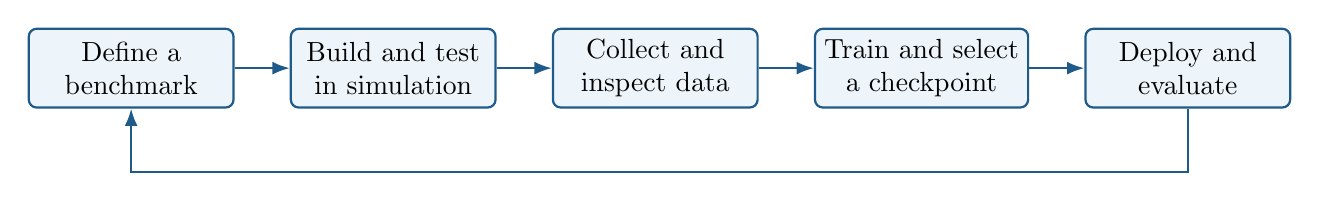
\begin{tikzpicture}[
  node distance=8mm and 7mm,
  box/.style={draw=lirmmblue,rounded corners=1mm,thick,align=center,
              minimum height=10mm,minimum width=26mm,fill=softblue},
  arr/.style={-{Latex[length=2.2mm]},thick,lirmmblue}
]
  \node[box] (task) {Define a\\benchmark};
  \node[box,right=of task] (sim) {Build and test\\in simulation};
  \node[box,right=of sim] (data) {Collect and\\inspect data};
  \node[box,right=of data] (train) {Train and select\\a checkpoint};
  \node[box,right=of train] (deploy) {Deploy and\\evaluate};
  \draw[arr] (task) -- (sim);
  \draw[arr] (sim) -- (data);
  \draw[arr] (data) -- (train);
  \draw[arr] (train) -- (deploy);
  \draw[arr] (deploy.south) |- ++(0,-8mm) -| (task.south);
\end{tikzpicture}%
}
\end{center}

Each stage should produce evidence before the next one starts. A scene that
loads is not yet a valid benchmark; a dataset that has the expected shape is
not necessarily useful; a low validation loss is not proof of closed-loop task
success; and a robot that moves is not yet a safe deployment.

\begin{methodbox}[General rule]
Change one source of difficulty at a time. Begin with a task that is easy to
interpret, then add position, orientation, lighting, object, or geometry
variation progressively. When several variables change together, a failure is
hard to diagnose and the next dataset is difficult to design.
\end{methodbox}

\section{Define success before writing code}

A benchmark description should answer five questions:

\begin{enumerate}
  \item What is the initial state distribution?
  \item What observations are available to the policy?
  \item What actions can the policy command?
  \item What event counts as success or failure?
  \item Which conditions remain fixed during one evaluation?
\end{enumerate}

Avoid descriptions such as ``the robot should usually grasp the object.'' A
useful definition is observable: for example, ``the object starts inside a
marked region and the trial succeeds when it is released inside the target box
without triggering a safety stop.'' Also define a maximum duration and the
handling of contacts, re-grasps, human intervention, and sensor failure.

\begin{projectbox}[Internship example]
The project moved from simulation to a simple physical pick-and-drop task, then
to constrained extraction with progressively larger pose variation. Each stage
added one observable difficulty while retaining the same experimental cycle.
\end{projectbox}

\section{Separate interfaces from implementations}

A learned policy should be treated as one component with a clear contract:

\begin{equation}
  \text{recent observations} \longrightarrow
  \text{future action sequence}.
\end{equation}

The simulator and physical robot do not need the same internal code, but they
must provide compatible concepts: camera images, robot state, action decoding,
and timing. Keeping these interfaces explicit makes it possible to replace the
model architecture or manipulator without rewriting the complete workflow.

Simulation can validate the method and interfaces without implying direct
transfer of one trained model to the physical robot. Decide explicitly whether
simulation data, model weights, or only software interfaces will be reused.

\section{What should remain reproducible}

For every dataset, training run, and evaluation, record at least:

\begin{itemize}
  \item exact code version (the result of \filepath{git rev-parse HEAD}) and
  configuration values used for the run;
  \item task definition and object-pose range;
  \item camera placement, crop, resolution, and exposure mode;
  \item robot start state and control mode;
  \item observation and action definitions;
  \item number of accepted demonstrations;
  \item selected checkpoint and deployment parameters;
  \item individual evaluation trials, not only the final percentage.
\end{itemize}

The exact command is part of the experiment. A checkpoint filename alone is
insufficient because horizons, camera preprocessing, action convention, and
safety limits may be supplied at runtime.

\begin{checkpointbox}[Before continuing]
Write a one-page benchmark protocol and draw the observation/action interface.
If success, variation, and action semantics are still ambiguous, do not begin a
large data collection.
\end{checkpointbox}

\section{What MuJoCo Executes}
\label{sec:mujoco-concepts}

MuJoCo is a physics engine for articulated systems, contacts, and rigid-body
dynamics. A typical program has four steps:

\begin{center}
\begin{tikzpicture}[
  node distance=8mm and 8mm,
  box/.style={draw=lirmmblue,rounded corners=1mm,thick,align=center,
              minimum height=10mm,minimum width=29mm,fill=softblue},
  arr/.style={-{Latex[length=2.2mm]},thick,lirmmblue}
]
  \node[box] (xml) {MJCF/XML\\scene};
  \node[box,right=of xml] (model) {Compile to\\\filepath{MjModel}};
  \node[box,right=of model] (data) {Create\\\filepath{MjData}};
  \node[box,right=of data] (step) {Set control and\\call \filepath{mj_step}};
  \draw[arr] (xml) -- (model);
  \draw[arr] (model) -- (data);
  \draw[arr] (data) -- (step);
\end{tikzpicture}
\end{center}

The distinction between model and data is fundamental:

\begin{description}
  \item[\filepath{mujoco.MjModel}:] the compiled, mostly fixed description of
  bodies, joints, masses, geometry, cameras, actuators, and limits.
  \item[\filepath{mujoco.MjData}:] the changing state of one simulation,
  including joint position, velocity, control input, contact information, body
  pose, and simulation time.
  \item[\filepath{mujoco.mj_step}:] advances dynamics by one model time step.
  \item[\filepath{mujoco.mj_forward}:] recomputes derived positions and
  velocities after state was changed directly, without advancing time.
\end{description}

An XML edit requires the model to be reloaded. In contrast, moving a free object
at reset normally modifies \filepath{MjData} and then calls
\filepath{mj_forward}.

\section{Run the Minimal Example}

The repository contains a small example independent of the microwave task:

\begin{itemize}
  \item \filepath{dp_mujoco/examples/minimal_scene.xml};
  \item \filepath{dp_mujoco/examples/mujoco_basics.py}.
\end{itemize}

It contains a floor, light, one actuated hinge, a free cube, a site, and a
camera. Run it without graphics first:

\begin{lstlisting}[language=bash]
python dp_mujoco/examples/mujoco_basics.py
\end{lstlisting}

The output reports the simulation time step and the dimensions \filepath{nq},
\filepath{nv}, and \filepath{nu}, then prints the changing joint position and
control target. Open the same example interactively with:

\begin{lstlisting}[language=bash]
python dp_mujoco/examples/mujoco_basics.py --viewer --duration 10
\end{lstlisting}

The blue arm follows a sinusoidal target, the green cube falls under gravity,
and the red site follows the end of the arm. This one scene demonstrates
actuation, free-body dynamics, contact, and a kinematic reference frame.

\section{Read a Small MJCF Scene}

MJCF describes a hierarchy. Child bodies move with their parent, while joints
define the motion allowed between them. The important elements are:

\begin{table}[H]
  \centering
  \begin{tabularx}{\textwidth}{@{}p{0.20\textwidth}X@{}}
    \toprule
    \textbf{Element} & \textbf{Purpose} \\
    \midrule
    \filepath{body} & A rigid frame that can contain joints, geometry, sites, and child bodies. \\
    \filepath{joint} & One degree of freedom such as a hinge or slide. \\
    \filepath{freejoint} & Six free degrees of freedom, represented by 3D position and a quaternion. \\
    \filepath{geom} & Visual and/or collision geometry with size, mass, friction, and material. \\
    \filepath{site} & A massless reference frame used for a TCP, sensor location, or target. \\
    \filepath{camera} & A fixed or body-mounted viewpoint used by the viewer or renderer. \\
    \filepath{actuator} & Converts a value in \filepath{data.ctrl} into force, velocity, or position control. \\
    \bottomrule
  \end{tabularx}
\end{table}

The core of the tutorial scene is deliberately small:

\begin{lstlisting}[language=XML]
<body name="arm" pos="0 0 0.08">
  <joint name="arm_hinge" type="hinge" axis="0 1 0"
         range="-1.57 1.57"/>
  <geom type="capsule" fromto="0 0 0 0 0 0.35"
        size="0.025" mass="0.5"/>
  <site name="tool_site" pos="0 0 0.35" size="0.015"/>
</body>

<actuator>
  <position name="arm_position" joint="arm_hinge" kp="20"/>
</actuator>
\end{lstlisting}

The actuator type defines the meaning of \filepath{data.ctrl}. Here the value
is a desired hinge angle. A motor actuator would interpret it differently, so
never assume that \filepath{ctrl} always contains joint positions.

MuJoCo uses half-extents for a box \filepath{geom}: a box with
\filepath{size="0.04 0.04 0.04"} measures $8\times8\times8$~cm. Incorrectly
treating these values as full dimensions is a common source of collision errors.

\section{Understand the Python Simulation Loop}

The essential Python loop is:

\begin{lstlisting}[language=Python]
model = mujoco.MjModel.from_xml_path("minimal_scene.xml")
data = mujoco.MjData(model)

actuator_id = mujoco.mj_name2id(
    model, mujoco.mjtObj.mjOBJ_ACTUATOR, "arm_position"
)

while data.time < 4.0:
    data.ctrl[actuator_id] = target_angle
    mujoco.mj_step(model, data)
\end{lstlisting}

The most frequently inspected arrays are:

\begin{description}
  \item[\filepath{data.qpos}:] generalized positions. A hinge uses one value;
  a free joint uses seven values: three for position and four for orientation.
  \item[\filepath{data.qvel}:] generalized velocities. A free joint uses six
  values, so \filepath{nq} and \filepath{nv} need not be equal.
  \item[\filepath{data.ctrl}:] one input per actuator; its length is
  \filepath{model.nu}.
  \item[\filepath{data.site_xpos/site_xmat}:] world position and orientation of
  sites after forward kinematics or a simulation step.
\end{description}

Use names instead of hard-coded indices when possible. The project obtains the
TCP site in the same way:

\begin{lstlisting}[language=Python]
site_id = mujoco.mj_name2id(
    model, mujoco.mjtObj.mjOBJ_SITE, "grasp_site"
)
tcp_position = data.site_xpos[site_id].copy()
\end{lstlisting}

\section{Open the Project Scene}
\label{sec:mujoco-scene}

The active task scene is:

\begin{center}
\filepath{dp_mujoco/models/universal_robots_ur10e/scene_microwave_camera.xml}
\end{center}

The scene includes \filepath{ur10e_with_gripper.xml}; this keeps robot links,
joints, gripper, actuators, wrist camera, and \filepath{grasp_site} separate
from the microwave, table, objects, target boxes, lighting, and global camera.
The Python files around the XML are:

\begin{table}[H]
  \centering
  \begin{tabularx}{\textwidth}{@{}p{0.42\textwidth}X@{}}
    \toprule
    \textbf{Path} & \textbf{Responsibility} \\
    \midrule
    \filepath{dp_mujoco/env/mujoco_env.py} & Loads the scene and exposes state, rendering, reset, and commands. \\
    \filepath{dp_mujoco/env/scene_utils.py} & Changes object pose during teleoperation resets. \\
    \filepath{dp_mujoco/utils/scene_utils.py} & Applies the matching reset distribution during policy execution. \\
    \filepath{dp_mujoco/teleop/test_UR10e_touch.py} & Runs simulated teleoperation and recording. \\
    \filepath{dp_mujoco/policy_exec/run_diffusion_mujoco.py} & Executes a trained checkpoint in MuJoCo. \\
    \bottomrule
  \end{tabularx}
\end{table}

Open the XML without ROS or the Touch:

\begin{lstlisting}[language=bash]
python -m mujoco.viewer \
  --mjcf=dp_mujoco/models/universal_robots_ur10e/scene_microwave_camera.xml
\end{lstlisting}

Inspect the body hierarchy, joint limits, contact geometry, and initial object
poses. The rendered mesh may look correct even when its collision geometry is
wrong, so enable contact or geometry visualization when debugging.

\section{Separate Visual and Collision Geometry}

A detailed mesh is useful for appearance but often unnecessarily difficult for
contact. In the project scene, the microwave OBJ mesh has collision disabled and
simple transparent boxes represent its floor, walls, and back. This makes
contact faster and easier to inspect.

When adding an object, begin with a primitive:

\begin{lstlisting}[language=XML]
<body name="practice_cube" pos="0.60 0.00 0.48">
  <freejoint/>
  <geom type="box" size="0.025 0.025 0.025"
        mass="0.10" rgba="0.15 0.55 0.90 1"/>
</body>
\end{lstlisting}

Reload the XML and let the object settle. If it falls through, jumps, or becomes
stuck, check units, initial overlap, collision dimensions, mass, friction, and
contact settings before modifying the robot controller.

\section{Render the Policy Cameras}

The project uses \filepath{top_table} as the global camera and
\filepath{wrist_cam} as the eye-in-hand camera. A renderer must be updated from
the latest \filepath{MjData} before an image is read:

\begin{lstlisting}[language=Python]
renderer = mujoco.Renderer(model, height=480, width=640)
renderer.update_scene(data, camera="top_table")
rgb_image = renderer.render()
\end{lstlisting}

\begin{figure}[H]
  \centering
  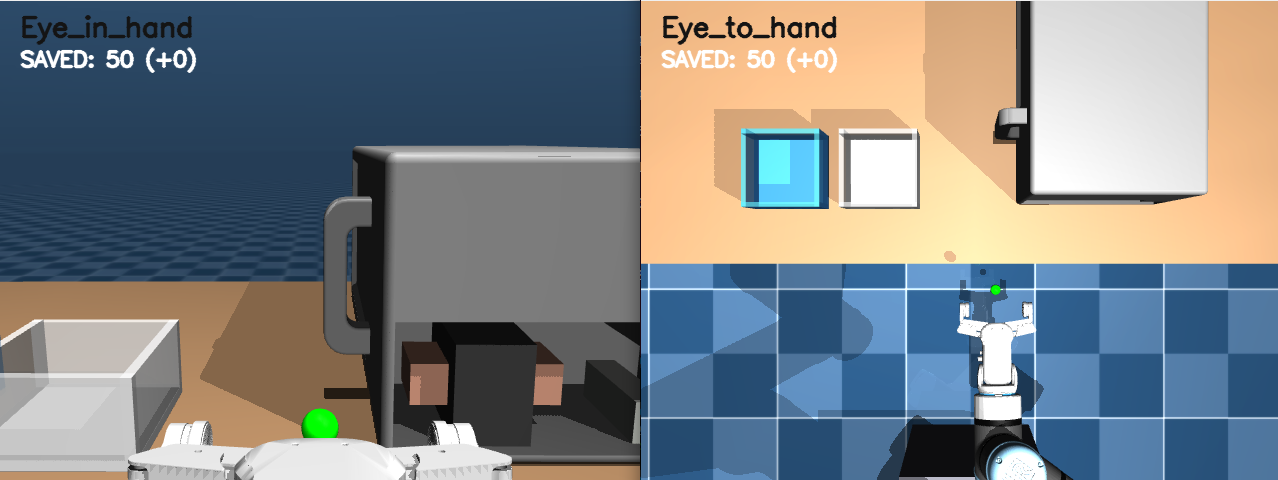
\includegraphics[width=0.86\textwidth]{camera_view.png}
  \caption{Project camera observations: wrist view on the left and global view on the right.}
  \label{fig:sim-camera-example}
\end{figure}

The teleoperation display uses $640\times480$ images, while its recorder resizes
them to $84\times84$ for the simulation dataset. Camera name, ordering,
orientation, and final image size must remain identical during policy execution.

\section{Reset and Randomize an Object}

A free joint stores object position followed by a quaternion in
\filepath{data.qpos}. The project reset utility finds the free-joint address,
writes the new pose, clears its six velocity values, and calls
\filepath{mj_forward}:

\begin{lstlisting}[language=Python]
qpos_adr = model.jnt_qposadr[joint_id]
qvel_adr = model.jnt_dofadr[joint_id]

data.qpos[qpos_adr:qpos_adr + 3] = position
data.qpos[qpos_adr + 3:qpos_adr + 7] = quat_wxyz
data.qvel[qvel_adr:qvel_adr + 6] = 0.0
mujoco.mj_forward(model, data)
\end{lstlisting}

The reset distribution used for collection and policy execution must match.
The current repository has one randomization module for each path; update and
test both when the pose range changes. Run many resets before recording and
confirm that every object pose is collision-free, visible, reachable, and part
of the intended task.

\begin{checkpointbox}[MuJoCo environment ready]
The minimal example runs, the project XML opens, the robot and free objects
behave correctly under gravity and contact, both cameras render useful views,
and repeated reset samples remain valid. Only then connect the Touch and test
the complete teleoperation loop.
\end{checkpointbox}

\chapter{Teleoperation and Data Recording}
\label{chap:touch}
\label{chap:collection}

Teleoperation is not only a convenient way to move the robot. It defines the
behavior that the policy will imitate. Controller lag, inconsistent gripper
commands, occlusion, and unnecessary corrective motions all become part of the
training target.

\section{A reusable teleoperation architecture}

A practical teleoperation system separates device input, target generation,
low-level control, and recording:

\begin{center}
\resizebox{\textwidth}{!}{%
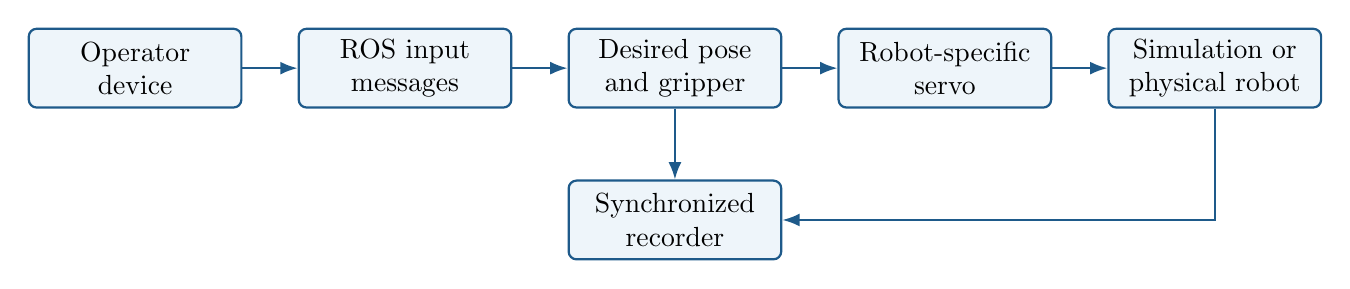
\begin{tikzpicture}[
  node distance=7mm and 7mm,
  box/.style={draw=lirmmblue,rounded corners=1mm,thick,align=center,
              minimum height=10mm,minimum width=27mm,fill=softblue},
  arr/.style={-{Latex[length=2.2mm]},thick,lirmmblue}
]
  \node[box] (device) {Operator\\device};
  \node[box,right=of device] (ros) {ROS input\\messages};
  \node[box,right=of ros] (target) {Desired pose\\and gripper};
  \node[box,right=of target] (servo) {Robot-specific\\servo};
  \node[box,right=of servo] (robot) {Simulation or\\physical robot};
  \node[box,below=9mm of target] (record) {Synchronized\\recorder};
  \draw[arr] (device) -- (ros);
  \draw[arr] (ros) -- (target);
  \draw[arr] (target) -- (servo);
  \draw[arr] (servo) -- (robot);
  \draw[arr] (robot.south) |- (record.east);
  \draw[arr] (target.south) -- (record.north);
\end{tikzpicture}%
}
\end{center}

This separation makes the input device and learned-policy interface reusable.
Only the servo and state reader must change for another robot.

\begin{projectbox}[Implementation used during the internship]
The 3D Systems Touch publishes pose and buttons through a ROS~2 C++ node. A
Python listener converts incremental stylus motion into a Cartesian target.
Pinocchio computes forward kinematics and the Jacobian
\citep{carpentier2019pinocchio}. The same target logic feeds either MuJoCo or a
UR10 \filepath{speedj} backend.
\end{projectbox}

\section{Use relative motion, not device coordinates}

The physical coordinates of a desktop device generally have no useful absolute
relationship with the robot base. Use differential motion:

\begin{equation}
  \Delta p_{robot} = s_p M_p
  \left(p^{device}_{t}-p^{device}_{t-1}\right),
\end{equation}

where $M_p$ maps axes and $s_p$ sets workspace scale. The first valid device
pose becomes a reference and produces no robot movement. This prevents the
initial jump that would occur if the device pose were interpreted as an
absolute robot target.

Test one translation and one rotation axis at a time. If an axis is wrong,
correct the mapping rather than teaching the operator to compensate mentally.

\section{From target error to robot motion}

For Cartesian velocity control, a common structure is:

\begin{equation}
  v_{des} =
  \begin{bmatrix}K_p e_p & K_r e_r\end{bmatrix}^{T},
  \qquad
  \dot q = J^{\#}(q)v_{des},
\end{equation}

where $e_p$ and $e_r$ are pose errors and $J^{\#}$ is a damped pseudoinverse.
Joint velocity and acceleration limits must be applied after this conversion.

Target smoothing can reduce abrupt hand motion:

\begin{equation}
  x_f(t)=(1-\alpha)x_f(t-1)+\alpha x_{raw}(t).
\end{equation}

A large $\alpha$ is responsive but transmits more noise; a small $\alpha$ is
smooth but introduces lag. Tune scale, target-speed limit, filter alpha, servo
gain, and joint limit one at a time. Several different parameter combinations
can produce similar slow motion while having very different behavior near
contact.

\section{Understand the timing chain}

The device, controller, cameras, and recorder do not need the same frequency.
For example, the internship setup approximately used:

\begin{table}[H]
  \centering
  \caption{Typical rates in the real teleoperation pipeline.}
  \begin{tabular}{@{}ll@{}}
    \toprule
    \textbf{Process} & \textbf{Reference rate} \\
    \midrule
    Touch ROS~2 publication & approximately 100 Hz \\
    Robot control loop & 50 Hz \\
    RealSense capture & 30 Hz \\
    Demonstration recording & 10 Hz \\
    \bottomrule
  \end{tabular}
\end{table}

The controller should consume the newest available target, while the recorder
periodically samples a coherent observation-action pair. Queueing every old
device message increases lag without adding useful information.

\begin{methodbox}[Measure latency instead of guessing]
Timestamp device input, camera capture, target generation, command transmission,
and recorder write. Log dropped or stale frames. A slow response may come from
the ROS path, camera blocking, controller filtering, disk compression, or the
robot safety slider; increasing $K_p$ does not fix all of these causes.
\end{methodbox}

Useful improvements for a future implementation are:

\begin{itemize}
  \item use depth-one/latest-sample ROS QoS for interactive targets;
  \item capture cameras continuously rather than starting a blocking read in
  the servo loop;
  \item move image compression and Zarr writes to a bounded background queue;
  \item record timestamps and reject a sample when one camera is stale;
  \item display control error, frame age, and saved-step count to the operator;
  \item stop or invalidate the episode after a frozen camera rather than saving
  apparently normal repeated images.
\end{itemize}

\section{Design the gripper command as part of the task}

Continuous gripper measurements are not always good action labels. A physical
gripper moves slowly and may report different intermediate widths for the same
operator intention. If the task naturally uses semantic states, record the
commanded state as the action and the measured width as an observation.

In the internship dataset, the gripper action used three semantic states
(open, narrow, and grasp). The narrowed state allowed entry into the cavity.
The commanded state was stored in \filepath{action}, while measured opening was
stored in \filepath{robot0_gripper_qpos}; this preserved operator intention and
still exposed actuator delay.

Use continuous commands when the task genuinely requires variable grasp width.
Do not quantize only to hide inconsistent data; choose an action representation
that matches the future task.

\section{Collect demonstrations that teach observable corrections}

A good demonstration is not simply a successful one. It should make the reason
for each correction visible to the policy. Practical recommendations are:

\begin{itemize}
  \item practice the controller before recording;
  \item begin and end episodes close to the useful task interval;
  \item use a consistent phase order and start configuration;
  \item avoid moving from information that is visible only to the human;
  \item delay fine alignment until the relevant camera sees the object;
  \item avoid passing the gripper in front of the object unnecessarily;
  \item cancel failed, interrupted, or camera-corrupted demonstrations;
  \item include deliberate coverage of the expected pose range.
\end{itemize}

In the constrained-extraction experiments, early demonstrations sometimes
began orientation corrections before the wrist camera clearly saw the component. Later
demonstrations approached first, waited for a useful wrist view, and then
aligned. This made the observation-action relationship easier to learn.

\section{Launch through maintained wrappers}

The repository uses \filepath{launch_all.sh} for simulation and
\filepath{ur10_real_robot/run_teleop.sh} for physical collection. The complete
commands and controls are maintained in \filepath{README_CODE.md}. On another
platform, replace the robot adapter and limits while preserving the staged
pre-flight, recording, and dataset checks.

\begin{safetybox}[Physical teleoperation]
An operator must be trained on the platform, the speed slider must begin low,
the workspace must be clear, and an emergency stop must remain reachable. Test
each mapped axis with millimetric motions before combining directions or
recording data.
\end{safetybox}

\begin{checkpointbox}[Before a long collection]
Record three episodes, replay every frame, plot the trajectory, and verify the
gripper labels. Continue only if the motion is responsive enough for small
corrections and the saved data represents what the operator intended.
\end{checkpointbox}

\chapter{Record and Check Demonstrations}
\label{chap:data}

The MuJoCo teleoperation program records complete task attempts as episodes in a
Zarr dataset. Recording and control occur in the same program, so the saved
images, measured state, and demonstrated target share one timeline.

\section{Record Episodes}

Start \filepath{./launch_all.sh} as described in \cref{chap:touch}. The MuJoCo
window uses these controls:

\begin{table}[H]
  \centering
  \begin{tabular}{@{}ll@{}}
    \toprule
    \textbf{Key} & \textbf{Action} \\
    \midrule
    \filepath{Space} & Start recording; press again to stop and save the episode. \\
    \filepath{Backspace} & Cancel the current episode without saving it. \\
    \filepath{R} & Reset the robot and randomize the scene. \\
    \filepath{Esc} & Quit. \\
    \bottomrule
  \end{tabular}
\end{table}

The recorder creates a timestamped dataset under \filepath{data/datasets/} and
samples at 10~Hz. Practice before recording. Start just before useful motion,
finish after task completion, and cancel failed, interrupted, or corrupted
attempts rather than teaching them as intended behavior.

\section{Define one synchronized sample}

A visuomotor sample normally contains:

\begin{equation}
  \left(o_t, a_t\right)
  = \left(\text{images}_t,\text{robot state}_t,
  \text{demonstrated command}_t\right).
\end{equation}

An episode is the ordered sequence from one start/stop interval. Episode
boundaries must remain intact because a training window must never cross from
the end of one attempt into the reset of the next.

\section{Define and document the schema}

The exact keys are project-specific. For example, the internship recorder
stored the following Zarr arrays at 10 Hz:

\begin{table}[H]
  \centering
    \caption{MuJoCo dataset interface used by the project recorder.}
  \begin{tabularx}{\textwidth}{@{}p{0.34\textwidth}p{0.20\textwidth}X@{}}
    \toprule
    \textbf{Key} & \textbf{Per-step shape} & \textbf{Meaning} \\
    \midrule
    \filepath{agentview_image} & $84\times84\times3$ & Global RGB image. \\
    \filepath{robot0_eye_in_hand_image} & $84\times84\times3$ & Wrist RGB image. \\
    \filepath{robot0_eef_pos} & 3 & Measured end-effector position. \\
    \filepath{robot0_eef_quat} & 4 & Measured end-effector quaternion. \\
    \filepath{robot0_gripper_qpos} & 1 & Measured gripper opening/state. \\
    \filepath{action} & 8 & Target pose and gripper command. \\
    \bottomrule
  \end{tabularx}
\end{table}

The simulation action is

\begin{equation}
  a_t=[x,y,z,q_x,q_y,q_z,q_w,g].
\end{equation}

The quaternion stored in the action is \filepath{xyzw}; the measured
\filepath{robot0_eef_quat} observation is \filepath{wxyz}. This project-specific
difference is handled by the current recorder and runner, but must not be
silently changed or mixed with real-robot datasets.

\section{Inspect structure, content, and coverage}

Validate every new dataset before sending it to the training server.

First confirm episode count, equal array lengths, action dimension, image
shapes, and valid Zarr structure:

\begin{lstlisting}[language=bash]
python scripts/check_zarr.py data/datasets/<dataset>.zarr
\end{lstlisting}

Then replay every episode and inspect the robot trajectory:

\begin{lstlisting}[language=bash]
python scripts/replay_zarr.py data/datasets/<dataset>.zarr --scale 2
python scripts/traj_zarr.py data/datasets/<dataset>.zarr
\end{lstlisting}

Look for frozen or repeated images, long idle intervals, abrupt target jumps,
unintended corrective loops, incorrect gripper transitions, and actions that
cannot be explained from the recorded observations. Also verify that object
positions and orientations cover the range expected during policy execution.

\begin{methodbox}[Demonstration quality]
A successful episode is not automatically a good demonstration. Keep motions
deliberate and consistent, avoid hiding the object at critical moments, and
cancel an episode when the operator makes a correction that should not be
imitated. Record three episodes first and inspect all of them before continuing
with a long session.
\end{methodbox}

Keep the original dataset immutable after training begins. If episodes must be
removed or new demonstrations added, create a new named version so that each
checkpoint can still be linked to the data that produced it.

\begin{checkpointbox}[Interface freeze]
The structure checker passes, every accepted episode has been replayed, camera
frames remain live, actions match operator intent, and the demonstrated pose
range matches the task that will be tested.
\end{checkpointbox}

\section{Train and Select a Model on Shared Compute}
\label{chap:training}

Training should begin only after the dataset interface has been frozen and a
small end-to-end smoke test has succeeded. The goal of the server workflow is
not merely to obtain a checkpoint; it is to preserve enough information to
reproduce how that checkpoint was produced.

\subsection{Freeze one training configuration}

Record the following before launching a long run:

\begin{itemize}
  \item dataset path and episode count;
  \item observation keys, shapes, and preprocessing;
  \item action representation and horizons;
  \item model architecture and parameter count;
  \item optimizer, learning rate, scheduler, batch size, and seed;
  \item train/validation split by episode;
  \item number of epochs and checkpoint interval;
  \item software revision and training device.
\end{itemize}

For a new model, first train for only a few batches and load the resulting
checkpoint in the policy runner. This verifies configuration composition,
tensor shapes, normalization, and serialization before consuming hours of GPU
time.

\subsection{Keep execution contexts explicit}

Distinguish the local experiment PC, server host, container, and Python
environment. Many path and import errors come from running a correct command in
the wrong context; for example, \filepath{/workspace} exists inside the project
container, not on the local robot computer.

\subsection{A general server workflow}

\begin{enumerate}
  \item Validate the dataset and record the source revision.
  \item Transfer only the required source, configuration, and data.
  \item Use a persistent session and a documented container/environment.
  \item Print resolved paths and run a short smoke test.
  \item Monitor the run and copy model candidates with their configurations
  back to the deployment computer.
\end{enumerate}

Use a persistent container or a documented image. Installing arbitrary packages
interactively until an import works makes the next run difficult to reproduce.

\subsection{Example: LIRMM training setup}

\begin{projectbox}[Internship example]
Training ran on \filepath{mic-gpu1} inside a persistent Docker container using
one NVIDIA A100 GPU. Data and configurations were transferred with
\filepath{rsync}; \filepath{tmux} protected the run from SSH disconnection. An
absolute dataset path was supplied explicitly, and the trained model was loaded
on the local CPU before robot testing. Exact server and training commands are in
\filepath{README_SERVER.md}.
\end{projectbox}

\subsection{What to monitor}

Monitor several signals rather than one number:

\begin{description}
  \item[Training loss:] confirms that the optimizer can fit the demonstrations.
  \item[Validation loss:] detects generalization degradation on held-out episodes.
  \item[Action error or samples:] helps reveal one problematic action component.
  \item[GPU use and step time:] reveals data-loader, memory, or device problems.
  \item[Closed-loop rollouts:] measure the behavior that ultimately matters.
\end{description}

The first Zarr load may be slow because chunks are decompressed and cached. A
pause after model construction is not proof that training has frozen; inspect
CPU, disk, GPU, and process activity before interrupting it.

\subsection{Select model candidates}

Save model candidates often enough to observe overfitting. Validation loss may
reach its minimum early, while closed-loop performance does not always rank
candidates in exactly the same order.

A sensible selection procedure is:

\begin{enumerate}
  \item reject runs with unstable or inconsistent training;
  \item choose a small set around the best validation region;
  \item benchmark inference time and load each checkpoint locally;
  \item test candidates in simulation or a no-motion real stage;
  \item choose one checkpoint before the reported evaluation trials.
\end{enumerate}

Do not change the selected model during the final evaluation. Development
trials and evaluation trials have different roles.

\subsection{Typical failures}

\begin{longtable}{@{}p{0.29\textwidth}p{0.65\textwidth}@{}}
  \toprule
  \textbf{Symptom} & \textbf{First checks} \\
  \midrule
  \endhead
  Dataset not found & Print the path inside the container; verify mount, transfer location, and Hydra-resolved value. \\
  CUDA out of memory & Check other processes, selected GPU, batch size, workers, image resolution, and model size. \\
  Training appears frozen & Inspect first-load caching, disk activity, workers, shared memory, and GPU utilization. \\
  Loss becomes NaN & Check normalization, invalid actions, learning rate, mixed precision, and exploding gradients. \\
  Validation rises early & Check split size, dataset diversity, augmentation, checkpoint frequency, and overfitting. \\
  Checkpoint fails locally & Check source revision, policy class, preprocessing, dependency compatibility, and EMA loading. \\
  \bottomrule
\end{longtable}

\begin{checkpointbox}[Training output]
For every candidate checkpoint, keep the resolved configuration, dataset name,
Git revision, epoch, validation metrics, parameter count, and a measured
inference latency on the deployment computer.
\end{checkpointbox}

\chapter{Deploying a Policy on a Robot}
\label{chap:deployment}

Deployment connects a statistical model to a safety-critical dynamical system.
Treat it as an interface and validation problem, not as one command that changes
\filepath{device=cpu} to \filepath{device=cuda}.

\section{Implement a robot adapter}

For a new robot, isolate four responsibilities:

\begin{enumerate}
  \item build observations in the exact training format;
  \item load normalization and run the policy;
  \item decode predicted actions into Cartesian or joint targets;
  \item enforce low-level control limits and stop conditions.
\end{enumerate}

The policy should not directly open sockets, read cameras, or implement robot
kinematics. A robot-specific adapter makes it possible to reuse the same policy
runner and replace only state acquisition and command execution.

\begin{projectbox}[UR10 implementation]
\filepath{ur10_real_robot/policy_exec/} contains the observation builder and
real runner. The backend reads UR10 state, two RealSense cameras, and gripper
width; a Pinocchio Cartesian servo converts pose targets to bounded joint
velocities; the gripper uses a Modbus adapter.
\end{projectbox}

\section{Deploy in stages}

Never begin with unrestricted physical motion. Use at least these stages:

\begin{description}
  \item[1. Offline/fake:] load the checkpoint, create correctly shaped dummy
  observations, and inspect predicted actions.
  \item[2. Real observations, no motion:] connect cameras and state readers,
  run inference, and print targets while commands remain disabled.
  \item[3. Low-speed physical motion:] use conservative limits, one object pose,
  a clear workspace, and an operator ready to stop.
  \item[4. Frozen evaluation:] fix checkpoint and parameters, then execute the
  written protocol.
\end{description}

At each stage, compare current observations with training data and verify units,
frames, quaternion order, TCP offset, action horizon, and gripper convention.

\section{Synchronous and asynchronous inference}

If inference is slower than action execution, synchronous replanning causes the
robot to pause while each new sequence is predicted. Asynchronous execution can
hide this delay:

\begin{figure}[H]
  \centering
  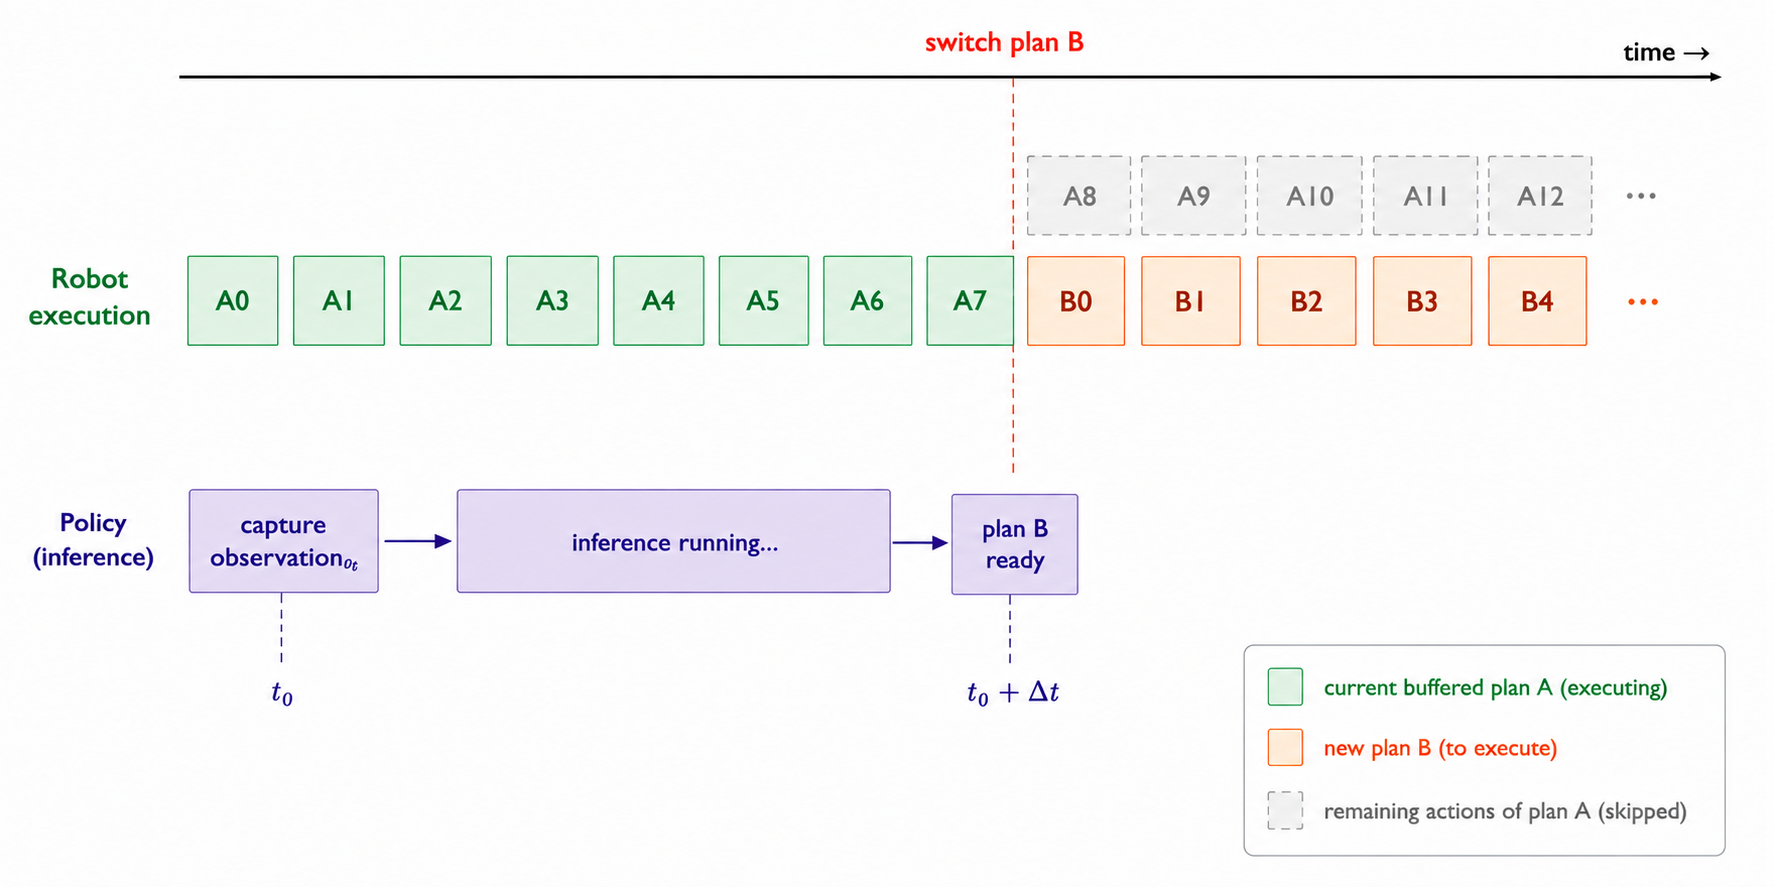
\includegraphics[width=0.96\textwidth]{asynchronous_inference_timeline.png}
  \caption{Asynchronous receding-horizon execution. The current buffered plan
  continues while the next plan is computed, then execution switches when the
  new plan is ready.}
  \label{fig:async-manual}
\end{figure}

This improves continuity but does not remove latency. The new plan is based on
an observation captured before inference began, so it may already be stale when
execution starts. Faster robot motion, longer inference, and contact-rich tasks
increase this mismatch.

Measure:

\begin{itemize}
  \item policy inference latency and its variance;
  \item age of the observation used for each plan;
  \item remaining actions when a new plan becomes ready;
  \item target discontinuity at plan switches;
  \item camera and control-loop delays separately.
\end{itemize}

Possible improvements include a deployment accelerator, a smaller model, a
faster valid decoder or sampler, temporal ensembling, latency-aware action
selection, and blending compatible plan transitions. Revalidate behavior after
changing model-specific inference settings.

\section{Parameters have different responsibilities}

Do not tune every parameter as a generic ``speed'' control.

\begin{table}[H]
  \centering
  \caption{Main deployment parameter groups.}
  \begin{tabularx}{\textwidth}{@{}p{0.32\textwidth}X@{}}
    \toprule
    \textbf{Group} & \textbf{What it controls} \\
    \midrule
    Model decoding/sampling & Computation cost and output approximation. \\
    Action/execution horizon & How long one prediction is consumed before replacement. \\
    Action execution rate & Time spacing between buffered targets. \\
    Cartesian gains & How aggressively tracking error is corrected. \\
    Target smoothing & Discontinuity/noise versus response lag. \\
    Joint and Cartesian limits & Maximum physical motion allowed by software. \\
    Position/rotation stop thresholds & Maximum discrepancy accepted before stopping. \\
    Teach-pendant slider & Hardware-level scaling of physical speed. \\
    \bottomrule
  \end{tabularx}
\end{table}

Record both requested software limits and the teach-pendant slider. Two runs
with the same command but different slider values are not the same execution
condition.

\section{Safety stops should latch and explain themselves}

A stop should cancel motion, prevent the same invalid target from being sent
repeatedly, and print enough context to diagnose the cause. Useful checks include:

\begin{itemize}
  \item target position and orientation error;
  \item joint velocity and workspace limits;
  \item stale camera or robot state;
  \item excessive control-loop time;
  \item loss of robot or gripper communication;
  \item invalid or non-finite policy output.
\end{itemize}

Do not increase a threshold only because it interrupts a trial. First determine
whether the large error comes from a wrong frame, quaternion, delayed plan,
unreachable target, or genuine tracking lag.

\section{Camera and gripper behavior during deployment}

Use the same camera order, crop, resolution, and exposure strategy as training.
Warm up cameras before the first observation and reject stale frames. If the
scene requires auto-exposure, give the camera time to adapt in both
demonstrations and deployment.

Decode the gripper action using the same semantics used during recording. Log
raw policy output, post-processing, command sent, target width, and measured
width. This distinguishes policy hesitation from actuator delay or contact.

\section{Use a staged execution wrapper}

The repository wrapper \filepath{ur10_real_robot/run_diffusion_real.sh}
defaults to motion disabled and requires an explicit motion-enable confirmation.
Its validated project commands are in \filepath{README_CODE.md}. A new robot
adapter should expose equivalent fake, observation-only, and physical-motion
stages.

\begin{safetybox}[Learned policy execution]
A successful checkpoint load does not imply a safe target. Keep independent
software limits, robot safety configuration, low initial speed, an unobstructed
workspace, and an operator able to stop motion immediately.
\end{safetybox}

\begin{checkpointbox}[Ready for evaluation]
The selected checkpoint and command are frozen; camera images match the dataset;
timing has been measured; repeated low-speed trials show bounded tracking; and
every stop condition has been tested or reviewed.
\end{checkpointbox}

\section{Short Troubleshooting Order}

When execution fails, check the pipeline in the same order in which it was
built:

\begin{table}[H]
  \centering
  \begin{tabularx}{\textwidth}{@{}p{0.27\textwidth}X@{}}
    \toprule
    \textbf{Symptom} & \textbf{First check} \\
    \midrule
    Scene or reset is wrong & Open the XML alone; inspect initial state, contacts, and randomization. \\
    Teleoperation is delayed & Check Touch topics, newest-target handling, scaling, smoothing, and simulation rate. \\
    Dataset looks wrong & Replay the affected episode; inspect frozen images, episode boundaries, action jumps, and gripper labels. \\
    Checkpoint will not load & Match source version, task YAML, policy class, and Python dependencies. \\
    Policy moves to the wrong pose & Check image order, normalization, action frame, quaternion convention, and reset distribution. \\
    Real robot tracks poorly & Compare raw target with measured pose, then inspect latency, controller limits, and safety output. \\
    \bottomrule
  \end{tabularx}
\end{table}

Change one variable at a time and repeat the smallest test that can confirm the
cause. Do not collect a larger dataset until scene, teleoperation, recording,
and deployment interfaces have been checked.

\section{What to Leave for the Next Student}

Keep a short record containing the dataset path and episode count, matching
training configuration, selected checkpoint, exact execution command, observed
inference latency, and known failure cases. With those items and the three
repository README files, another student can repeat the workflow without
reconstructing it from terminal history.

\begin{checkpointbox}[Complete workflow]
The task is stable in MuJoCo, teleoperation is responsive, accepted episodes
have been replayed, the checkpoint matches the dataset interface, and the policy
has been executed successfully in simulation before any physical deployment.
\end{checkpointbox}


\appendix
\chapter{Touch and OpenHaptics Installation}
\label{app:openhaptics}

\begingroup
\small
\lstset{
  basicstyle=\ttfamily\footnotesize,
  aboveskip=0.4em,
  belowskip=0.4em
}

This appendix gives the complete device-specific installation used for the
3D Systems Touch. The validated stack is Ubuntu 22.04, ROS~2 Humble,
OpenHaptics 3.4, and Touch Driver 2025.12.10. Install the general local
environment from \filepath{README_ENV.md} first. Keep the Touch disconnected
until the driver installation is complete.

\section{Download and extract the vendor packages}

Download both Linux archives from the official 3D Systems support page:

\begin{center}
\url{https://support.3dsystems.com/s/article/OpenHaptics-for-Linux-Developer-Edition-v34?language=en_US}
\end{center}

\begin{itemize}
  \item \textbf{OpenHaptics Installer --- OpenHaptics for Linux v3.4};
  \item \textbf{Haptic Device Driver Installer --- Touch Device Driver
  v2025.12.10}.
\end{itemize}

Create a permanent working directory and extract both archives. The browser may
append a suffix such as \filepath{(1)} to a repeated download; adapt the archive
name when necessary.

\begin{lstlisting}[language=bash]
mkdir -p "$HOME/touch_driver"

tar -xzf "$HOME/Downloads/openhaptics_3.4-0-developer-edition-amd64.tar.gz" \
  -C "$HOME/touch_driver"
tar -xzf "$HOME/Downloads/TouchDriver_2025_12_10+1.tgz" \
  -C "$HOME/touch_driver"

ls "$HOME/touch_driver/TouchDriver_2025_12_10"
ls "$HOME/touch_driver/openhaptics_3.4-0-developer-edition-amd64"
\end{lstlisting}

Do not place these vendor archives inside the Git repository.

\section{Install dependencies and vendor software}

Install the build, terminal, and OpenGL dependencies required by the SDK and
its examples:

\begin{lstlisting}[language=bash]
sudo apt update
sudo apt install -y \
  build-essential freeglut3-dev libglu1-mesa-dev \
  libncurses5-dev mesa-utils
\end{lstlisting}

Install the Touch driver first. This copies the device libraries and installs
the USB permission rule:

\begin{lstlisting}[language=bash]
cd "$HOME/touch_driver/TouchDriver_2025_12_10"
sudo bash ./install_haptic_driver
sudo udevadm control --reload-rules
sudo udevadm trigger
\end{lstlisting}

Reconnect the Touch after this command. Reboot if requested. Then install the
OpenHaptics SDK:

\begin{lstlisting}[language=bash]
cd "$HOME/touch_driver/openhaptics_3.4-0-developer-edition-amd64"
sudo ./install
sudo ldconfig
\end{lstlisting}

The SDK installer places examples and documentation under
\filepath{/opt/OpenHaptics/Developer/3.4-0/}. The project also keeps the
extracted SDK root so that CMake can locate the exact headers and libraries.

\section{Configure the SDK path}

Define \filepath{OPENHAPTICS_ROOT} and verify the two files required by the
project build:

\begin{lstlisting}[language=bash]
export OPENHAPTICS_ROOT="$HOME/touch_driver/openhaptics_3.4-0-developer-edition-amd64"

test -f "$OPENHAPTICS_ROOT/usr/include/HD/hd.h" \
  && echo "OpenHaptics headers found"
test -f "$OPENHAPTICS_ROOT/usr/lib/libHD.so" \
  && echo "OpenHaptics HD library found"
\end{lstlisting}

Both messages must appear. Make the setting persistent for Bash terminals:

\begin{lstlisting}[language=bash]
echo 'export OPENHAPTICS_ROOT="$HOME/touch_driver/openhaptics_3.4-0-developer-edition-amd64"' \
  >> "$HOME/.bashrc"
source "$HOME/.bashrc"
\end{lstlisting}

For Zsh, add the same export line to \filepath{\textasciitilde/.zshrc} instead.

Some vendor executables may report missing legacy terminal libraries such as
\texttt{libtinfo.so.5} or \texttt{libncurses.so.5}. Install them only when that
error occurs:

\begin{lstlisting}[language=bash]
sudo apt install -y libtinfo5 libncurses5
\end{lstlisting}

\section{Validate the device before ROS}

Plug in the Touch. First compile and run the read-only vendor diagnostic:

\begin{lstlisting}[language=bash]
cd "$OPENHAPTICS_ROOT/opt/OpenHaptics/Developer/3.4-0/examples/HD/console/QueryDevice"
make
./QueryDevice
\end{lstlisting}

The program must identify the device, and the displayed pose and button values
must change when the stylus moves. If initialization fails, stop here and fix
the driver, USB connection, permissions, or missing library before using ROS.

Run the calibration example when the device requests calibration:

\begin{lstlisting}[language=bash]
cd "$OPENHAPTICS_ROOT/opt/OpenHaptics/Developer/3.4-0/examples/HD/console/Calibration"
make
./Calibration
\end{lstlisting}

Finally, an optional force-feedback test verifies bidirectional communication:

\begin{lstlisting}[language=bash]
cd "$OPENHAPTICS_ROOT/opt/OpenHaptics/Developer/3.4-0/examples/HD/console/FrictionlessSphere"
make
./FrictionlessSphere
\end{lstlisting}

Move the stylus gently; a virtual sphere should be perceptible. Keep a light
grip and stop immediately with \filepath{Ctrl+C} if the device behaves
unexpectedly.

\section{Build the project ROS~2 driver}

Activate Conda, ROS~2, and the SDK path before building the workspace:

\begin{lstlisting}[language=bash]
cd "$HOME/Stage_Lirmm/Diffusion-model-isaacsim"
conda activate microwave_dp
source /opt/ros/humble/setup.bash
export OPENHAPTICS_ROOT="$HOME/touch_driver/openhaptics_3.4-0-developer-edition-amd64"

cd ros2_WS
rosdep install --from-paths src --ignore-src -r -y
colcon build --symlink-install \
  --cmake-args -DOPENHAPTICS_ROOT="$OPENHAPTICS_ROOT"
source install/setup.bash
\end{lstlisting}

If the workspace was copied from another computer, old absolute paths may
remain in generated files. Remove only the generated directories and rebuild:

\begin{lstlisting}[language=bash]
cd "$HOME/Stage_Lirmm/Diffusion-model-isaacsim/ros2_WS"
rm -rf build install log
colcon build --symlink-install \
  --cmake-args -DOPENHAPTICS_ROOT="$OPENHAPTICS_ROOT"
source install/setup.bash
\end{lstlisting}

\section{Validate the ROS topics}

Start the Touch node in terminal 1:

\begin{lstlisting}[language=bash]
cd "$HOME/Stage_Lirmm/Diffusion-model-isaacsim"
conda activate microwave_dp
source /opt/ros/humble/setup.bash
source ros2_WS/install/setup.bash
ros2 launch touch_ros2_driver touch_rviz.launch.py
\end{lstlisting}

Inspect its outputs in terminal 2:

\begin{lstlisting}[language=bash]
source /opt/ros/humble/setup.bash
source "$HOME/Stage_Lirmm/Diffusion-model-isaacsim/ros2_WS/install/setup.bash"
ros2 topic hz /touch/pose
ros2 topic echo /touch/buttons
\end{lstlisting}

The pose must update continuously and both buttons must change the published
value. Stop both terminals with \filepath{Ctrl+C}. Do not continue to MuJoCo or
a physical robot if the topic freezes, the axes jump while the device is still,
or the node reports an OpenHaptics scheduler error.

\section{Daily use and common failures}

In every new terminal used with the Touch, activate the three software layers:

\begin{lstlisting}[language=bash]
cd "$HOME/Stage_Lirmm/Diffusion-model-isaacsim"
conda activate microwave_dp
source /opt/ros/humble/setup.bash
source ros2_WS/install/setup.bash
\end{lstlisting}

\begin{tabularx}{0.96\linewidth}{@{}>{\raggedright\arraybackslash}p{0.26\linewidth}>{\raggedright\arraybackslash}X@{}}
  \toprule
  \textbf{Symptom} & \textbf{Check} \\
  \midrule
  Device not detected & Reconnect USB, reload the udev rules, reboot, and run
  \filepath{QueryDevice} before ROS. \\
  Missing legacy terminal library & Install the two compatibility packages
  shown above. \\
  CMake cannot find \filepath{HD/hd.h} & Correct
  \filepath{OPENHAPTICS_ROOT}, then delete only \filepath{ros2_WS/build},
  \filepath{install}, and \filepath{log} before rebuilding. \\
  Scheduler or device-in-use error & Close other OpenHaptics examples and ROS
  nodes; only one process should own the device. \\
  ROS topics are absent & Source ROS~2 and \filepath{ros2_WS/install/setup.bash},
  then inspect the first terminal for a driver error. \\
  \bottomrule
\end{tabularx}

Only after the vendor diagnostics and ROS topics pass should the Touch be linked
to MuJoCo. Any later physical robot motion still requires the staged procedure
described in \cref{sec:physical-deployment}.

\endgroup


\end{document}
